\documentclass[a4paper,12pt,oneside,onecolumn,final]{book}
\usepackage{times}
\usepackage{thesisStyle}
\usepackage{setspace}
\usepackage{calc}
\usepackage{indentfirst}
\usepackage{xspace}
% for tables
\usepackage{hyperref}
%\usepackage{array}
%\usepackage{dcolumn}
\usepackage{multirow}
\usepackage{layout}
\usepackage{tabularx}
%\usepackage{natbib}
\usepackage{picinpar}
\usepackage[table]{xcolor}
\usepackage{math tools}
\usepackage[normalem]{ulem}

\usepackage{caption,subcaption}

% for maths
\usepackage{amsmath}
\usepackage{amssymb}
\usepackage{amsthm}
\usepackage{listings}
%\usepackage{theorem}
\lstset{ %
	numberstyle=\scriptsize,
	basicstyle=\scriptsize\ttfamily,
	breaklines=true,
	tabsize=2,
	columns=fullflexible,
	numbers=left,
	stepnumber=1
}

\newcommand{\figref}[1]{Figure \ref{#1}}
\newcommand{\tabref}[1]{Table \ref{#1}}
\newcommand{\eqnref}[1]{Equation \ref{#1}}

\newcommand{\realcount}{A}
\newcommand{\II}{\mathcal{II}}
\newcommand{\saml}{\widetilde{l}}
\newcommand{\samL}{\widetilde{L}}
\newcommand{\CI}{\mathcal{CI}}
\newcommand{\samCI}{\widetilde{\mathcal{CI}}}
\newcommand{\IT}{{I^T}}
\newcommand{\samIT}{\widetilde{I^T}}
\newcommand{\Dhat}{\widetilde{D}}
\newcommand{\m}{\text{-}}
\newcommand{\R}{\mathcal{R}_s}
\newcommand{\Rhat}{\overline{\mathcal{R}_s}}
\newcommand{\RhatD}{\overline{\mathcal{R}_b}_\prec}
\newcommand{\RhatBD}{\overline{\mathcal{R}_b}_\succ}
\newcommand{\RhatIC}{\overline{\mathcal{R}_b}_\pi}
\newcommand{\RhatR}{\overline{\mathcal{R}_b}_\times}

\newcommand{\circled}[1]{\raisebox{.5pt}{\textcircled{\raisebox{-.9pt} {#1}}}}

\newtheorem{guarantee}{\sc Guarantee}


% for graphics
\usepackage{color}
\usepackage{graphicx}
%\usepackage[tight,FIGBOTCAP,TABBOTCAP,hang]{subfigure}
\usepackage{rotating}
\usepackage{epsfig}
%\usepackage{slashbox}

% for algorithms
%\usepackage[plain,section]{algorithm}
\usepackage{algorithm}
\usepackage{algorithmic}

\newcommand{\stitle}[1]{\vspace*{0.5em}\noindent{\bf #1\/} }
\newcommand{\sstitle}[1]{\noindent{\bf \small #1\/}}

\usepackage[numbers]{natbib}




\newtheorem{thm}{Theorem}
\newtheorem{lemma}{Lemma}
\newtheorem{proposition}{Proposition}
\newtheorem{property}{Property}
\newtheorem{corollary}{Corollary}
\newtheorem{conjecture}{Conjecture}
\newtheorem{definition}{Definition}
\newtheorem{example}{Example}
\newtheorem{claim}{Claim}
\newtheorem{condition}{Condition}
\newtheorem{pruning}{Pruning}
\newtheorem{accepting}{Accepting}
\DeclareMathOperator{\argmax}{arg\,max}


\newcounter{enum}
\newenvironment{packed_enum}{
\begin{list}{R\arabic{enum}.}{
%\begin{list}{(\alph{enum})}{
  \setlength{\itemsep}{-1pt}
  \setlength{\parskip}{0.5pt}
  \setlength{\labelwidth}{30 pt}
  \setlength{\leftmargin}{20 pt}
  \setlength{\itemindent}{1pt}
  \usecounter{enum}}
}{\end{list}}



\newenvironment{packed_item}{
\begin{list}{$\bullet$}{
%\begin{list}{(\alph{enum})}{
\setlength{\itemsep}{-1pt}
  \setlength{\parskip}{0.5pt}
  \setlength{\labelwidth}{30 pt}
  \setlength{\leftmargin}{20 pt}
  \setlength{\itemindent}{1pt}
  %  \usecounter{enum}} 
   }
}{\end{list}}


\newenvironment{packed_enum_roman}{
\begin{list}{\roman{enum}.}{
  \setlength{\itemsep}{-0.5pt}
  \setlength{\parskip}{1pt}
  \setlength{\labelwidth}{30 pt}
  \setlength{\leftmargin}{15 pt}
  \setlength{\itemindent}{0pt}
  \usecounter{enum}}
}{\end{list}}


\newenvironment{packed_enum_num}{
\begin{list}{\arabic{enum}.}{
%\begin{list}{(\alph{enum})}{
  \setlength{\itemsep}{-0.5pt}
  \setlength{\parskip}{1pt}
  \setlength{\labelwidth}{30 pt}
  \setlength{\leftmargin}{15 pt}
  \setlength{\itemindent}{0pt}
    %\setlength{\itemindent}{-\labelwidth}
  %\setlength{\listparindent}{-40 pt}
  \usecounter{enum}}
}{\end{list}}

\newenvironment{packed_enum_num2}{
\begin{list}{\arabic{enum}.}{
%\begin{list}{(\alph{enum})}{
  \setlength{\itemsep}{-0.5pt}
  \setlength{\parskip}{1pt}
  \setlength{\labelwidth}{30 pt}
  \setlength{\leftmargin}{15 pt}
  \setlength{\itemindent}{0pt}
  \setcounter{enum}{2}
    %\setlength{\itemindent}{-\labelwidth}
  %\setlength{\listparindent}{-40 pt}
  %\usecounter{enum}
  }
}{\end{list}}

%
%\pagestyle{myheadings}
%\markright{Page Limit: 7 pages\hfill}



%%----------------------------------------------------------------------------%%
%%    Page layout                                                             %%
%%----------------------------------------------------------------------------%%

%% from setspace.sty: 1.5 spacing for 11pt font
%\renewcommand{\baselinestretch}{1.5}
%\doublespacing

%% from vmargin.sty
\setlength{\hoffset}{-1in}
\setlength{\voffset}{-1in}
\setlength{\footskip}{0.95in}
\setlength{\headsep}{0.2in}
\setlength{\topmargin}{0.69in}
\setlength{\headheight}{0\baselineskip}
\setlength{\oddsidemargin}{0.99in}
\setlength{\evensidemargin}{0.99in}
\setlength{\textwidth}{\paperwidth-\oddsidemargin-\evensidemargin}
\setlength{\textheight}{\paperheight-\topmargin-\headheight-\headsep-\footskip}
\setlength{\parskip}{1ex}
\setlength{\parindent}{1em}
\setlength{\partopsep}{5pt}



\newcommand{\select}{\ensuremath{\sigma}}
\newcommand{\project}{\ensuremath{\pi}}
\newcommand{\agg}{\ensuremath{\chi}}
\newcommand{\join}{\ensuremath{\Join}}
\newcommand{\union}{\ensuremath{\cup}}
\newcommand{\minus}{\ensuremath{-}}
\newcommand{\product}{\ensuremath{\times}}

%\hyphenation{user/deve-loper-friendly}

\renewcommand{\bibname}{References}
\let\oldbibliography\bibliography
\renewcommand{\bibliography}[1]{{
	\let\chapter\section
	\oldbibliography{#1}
}}
%%----------------------------------------------------------------------------%%
%%    Various environments                                                    %%
%%----------------------------------------------------------------------------%%

\makeatletter
\newcommand\refootnote[1]{%
  \def\@thefnmark{\ref{#1}}%
  \@makefnmark}
\makeatother
\begin{document}
%%---------------------%%


\newpage

\stitle {\underline{Proposed Outline of Research Plan and Methodology}}

\setcounter{page}{1}


Statistical inference is an important technique to express hypothesis and
reason about data in data analytical tasks.  
Today, many big data applications are based on
statistical inference.
Examples include topic modeling \cite{blei2003latent,Titov2008a},
sentiment analysis \cite{Titov2008b, Jo2011,tsm}, spam filtering \cite{spam}, to name a few.
Statistical inference has two major components: the formal
representation of a \emph{statistical model}~\cite{cox} and 
the development of corresponding accurate and efficient 
{\em inference algorithms}.
%One of most critical steps of statistical inference is to construct a
%\emph{statistical model} to formally represent the underlying statistical
%inference task .  
Currently, most scalable machine learning libraries (e.g. MLlib \cite{mllib}) 
contain popular, standard statistical models such as support vector machine, 
linear regression, and latent Dirichlet allocation (LDA) \cite{blei2003latent}, 
and provide programming interface to their inference algorithms.
%Constructing a statistical model is never trivial because a domain user may have to devise and
%implement many  different models before finding a promising one for a specific
%task.    
However, to carry out statistical inference on
customized models with big data, the user has to implement her own models and
inference codes on a distributed framework like Apache Spark
\cite{Zaharia:2010:SCC:1863103.1863113} and Hadoop \cite{hadoop}.
Developing inference code requires extensive knowledge in both statistical
inference and programming techniques in distributed frameworks.  Moreover,
model definitions, inference algorithms, and data processing tasks are all
mixed up in the resulting code, making it hard to debug and reason about.  For
even a slight alteration to the model in quest of the most promising one, the
model designer will have to re-derive the formulas and re-implement the
inference codes, which is tedious and error-prone. 

In this project, we propose InferSpark, a \emph{probabilistic programming
framework} on top of Spark.  Probabilistic programming is an emerging
paradigm that allows statistician and domain users to succinctly express a model
definition within a host programming language and transfers the burden of
implementing the inference algorithm from the user to the compilers and
runtime systems \cite{pp}.  For example, Infer.NET \cite{InferNET14} is a
probabilistic programming framework that extends C\#.  The user can express,
say, a Bayesian network in C\# and the compiler will generate code to perform
inference on it. Such code could be as efficient as the implementation of
the same inference algorithm carefully optimized by
an experienced programmer.

So far, the emphasis of probabilistic programming has been put on the
expressiveness of the languages and the development of efficient inference
algorithms (e.g., variational message passing \cite{vmp}, Gibbs sampling \cite{gibbs},
Metropolis-Hastings sampling \cite{mh}) to handle a wider range of statistical
models.  The issue of scaling out these frameworks, however, has not been
addressed.  For example, Infer.NET only works on a single machine.  
When we tried to use Infer.NET to train an LDA model of 96 topics and 9040-word
vocabulary on only 3\% of Wikipedia articles, the actual memory
requirement has already exceeded 512GB, the maximum memory of most commodity
servers today.
%Frequent swapping makes each iteration take xxx hrs
%(still running, > 2 hr). Infer .NET deals with the scaling problem by
%splitting the whole dataset into chunks that fit in memory and iteratively
%load and process the chunks. Using the batched training, each iteration still
%takes over 21 minutes.  
The goal of InferSpark is thus to bring 
probabilistic programming to Spark, a predominant distributed data
analytic platform, for carrying out statistical inference at scale. 
The InferSpark project will consist of two parts:

\begin{packed_enum}
	\item {\bf Extending Scala to support probabilistic programming.}
	In InferSpark, we extend Scala with probabilistic programming constructs
	to exploit its functional features. User can define customized models
	that are not available in ML libraries in a succint language. 
	As an example, \figref{fig:slda} shows the SLDA model, a non-standard
        graphical model not available in MLlib. While the actual Spark 
	implementation contains hundreds of lines of code, the model can be 
	specified in just 7 lines of InferSpark code according to our proposing syntax. The fact
	that both preprocessing and post-processing can be included in one Scala
	program substantially eases the development process. Carrying out
	statistical inference with InferSpark is simple and intuitive, and
	implicitly enjoys the distributed computing capability brought by Spark.

	\item {\bf Building an InferSpark compiler and a runtime system.}
	InferSpark will include a compiler to compile InferSpark models into
	Scala/Spark classes and objects that implement the inference algorithms
	with a set of API. The user can call the API from their Scala programs to
	specify the input (observed) data and query about the model (e.g. compute
	the expectation of some random variables or retrieve the parameters of the
	posterior distributions). The runtime system will be built on top of
	Apache Spark, which includes customized Spark libraries tuned for the
	inference algorithms.
		
\end{packed_enum}


\begin{figure}
	\centering
	\begin{subfigure}[b]{.2\textwidth}
		\includegraphics[width=\textwidth]{figs/slda.eps}
		\caption{Graphical Model}
		\label{fig:slda}
	\end{subfigure} \hfill
	\begin{subfigure}[b]{.72\textwidth}
		\begin{lstlisting}[breaklines=true]
@Model
class SLDA(K: Long, V: Long, alpha: Double, beta: Double) {
  val phi = for (i <- 0L until K) yield Dirichlet(beta, V)
  val theta = for (i <- ?) yield Dirichlet(alpha, K)
  val z = theta.map{theta => for (i <- ?) yield Categorical(theta)}
  val w = z.map(_.map(z => ?.map(_ => Categorical(phi(z)))))
}
		\end{lstlisting}
		\caption{Model definition in InferSpark}
		\label{fig:slda_model_def}
	\end{subfigure}
	\caption{SLDA model}
\end{figure}

%Currently, InferSpark supports Bayesian network models. Bayesian network
%is a major branch of probabilistic graphical model and it has already covered
%models like naive Bayes, LDA, TSM \cite{tsm}, etc.  The goal of this paper is to
%describe the workflow, architecture, and Bayesian network implementation of
%InferSpark.  We will open-source InferSpark and support other models (e.g.,
%Markov networks) afterwards.  

To the best of our knowledge, InferSpark is the first endeavor to bring 
probabilistic programming into the (big) data engineering domain.
Efforts like MLI \cite{mli} and SystemML \cite{systemml} all aim 
at easing the difficulty of developing \emph{distributed machine learning techniques} 
(e.g., stochastic gradient descent (SGD)).
InferSpark aims at easing the complexity of developing 
\emph{custom statistical models}, 
with domain experts, data scientists, statistician, and 
machine learning researchers as the target users.

\begin{figure*}[th]
	\centering
	\includegraphics[width=0.7\columnwidth]{figs/workflow3.eps}
	\caption{InferSpark Architecture}
	\label{fig:workflow}
\end{figure*}

%\KZ{My general feeling is that the running example is not made full use of.
%The discussion should be tightly coupled to the running example. E.g., when
%we talk about schedule, just present the schedule for the two coins.
%Some of the stuff here should go into implementation section.}

The proposed architecture of InferSpark is shown in \figref{fig:workflow}. An
InferSpark program is a mix of statistical model definition and ordinary user
code. The statistical model construction module separates the model part out
and transforms it into a model template. This template is then instantiated
with parameters and metadata collected at run time. The code generation module
produces the inference code for the instantiated model, which is then executed
on the InferSpark runtime system to produce the final inference result.

The project team will be divided into two sub-groups, one led by Hong Kong PI, 
one led by mainland PI.
Each of which will communicate and interact with each other on a regular basis. 
Each sub-group will have two research students.
The mainland sub-group, led by PI Zhu, a programming language and 
data mining expert, will focus on the probabilistic programming 
language design for InferSpark
and the implementation of InferSpark compiler.
The Hong Kong sub-group, led by PI Lo, a database and systems expert, 
will focus on the design and implementation of InferSpark runtime system.
In the first phase (6 months), all students will learn about the background and the knowledge (e.g., statistical inference, architecture of various big data systems) related to the project.
In the second phase (6 months), the students will work together to 
design the probabilistic programming language for InferSpark.
In the third phase (12 months), the students will work together to 
design and implement InferSpark compiler.
In the fourth phase (12 months), the students will work together to build InferSpark runtime system.
In the last phase (12 months), the students will carry out various testing and experiments.


%An InferSpark program is a mix of model definition and
%normal user code. The graphical network construction module separates the
%model part out, and transforms it into a graphical network template. This
%template is then instantiated with parameters and meta data from the input
%data at runtime by the code generation module, which produces the inference
%code and message passing graph (MPG). These are then executed on the GraphX 
%distributed engine to produce the final posterior distribution.


%InferSpark analyzes the Bayesian network defined by a special 
%scala-like program and
%automatically transforms the model definition into the GraphX implementation
%of VMP algorithm. After two stages of compilation, the runtime system 
%launches the VMP implementation and returns the inference results 
%through the query API.  

%
%
%\begin{figure}
%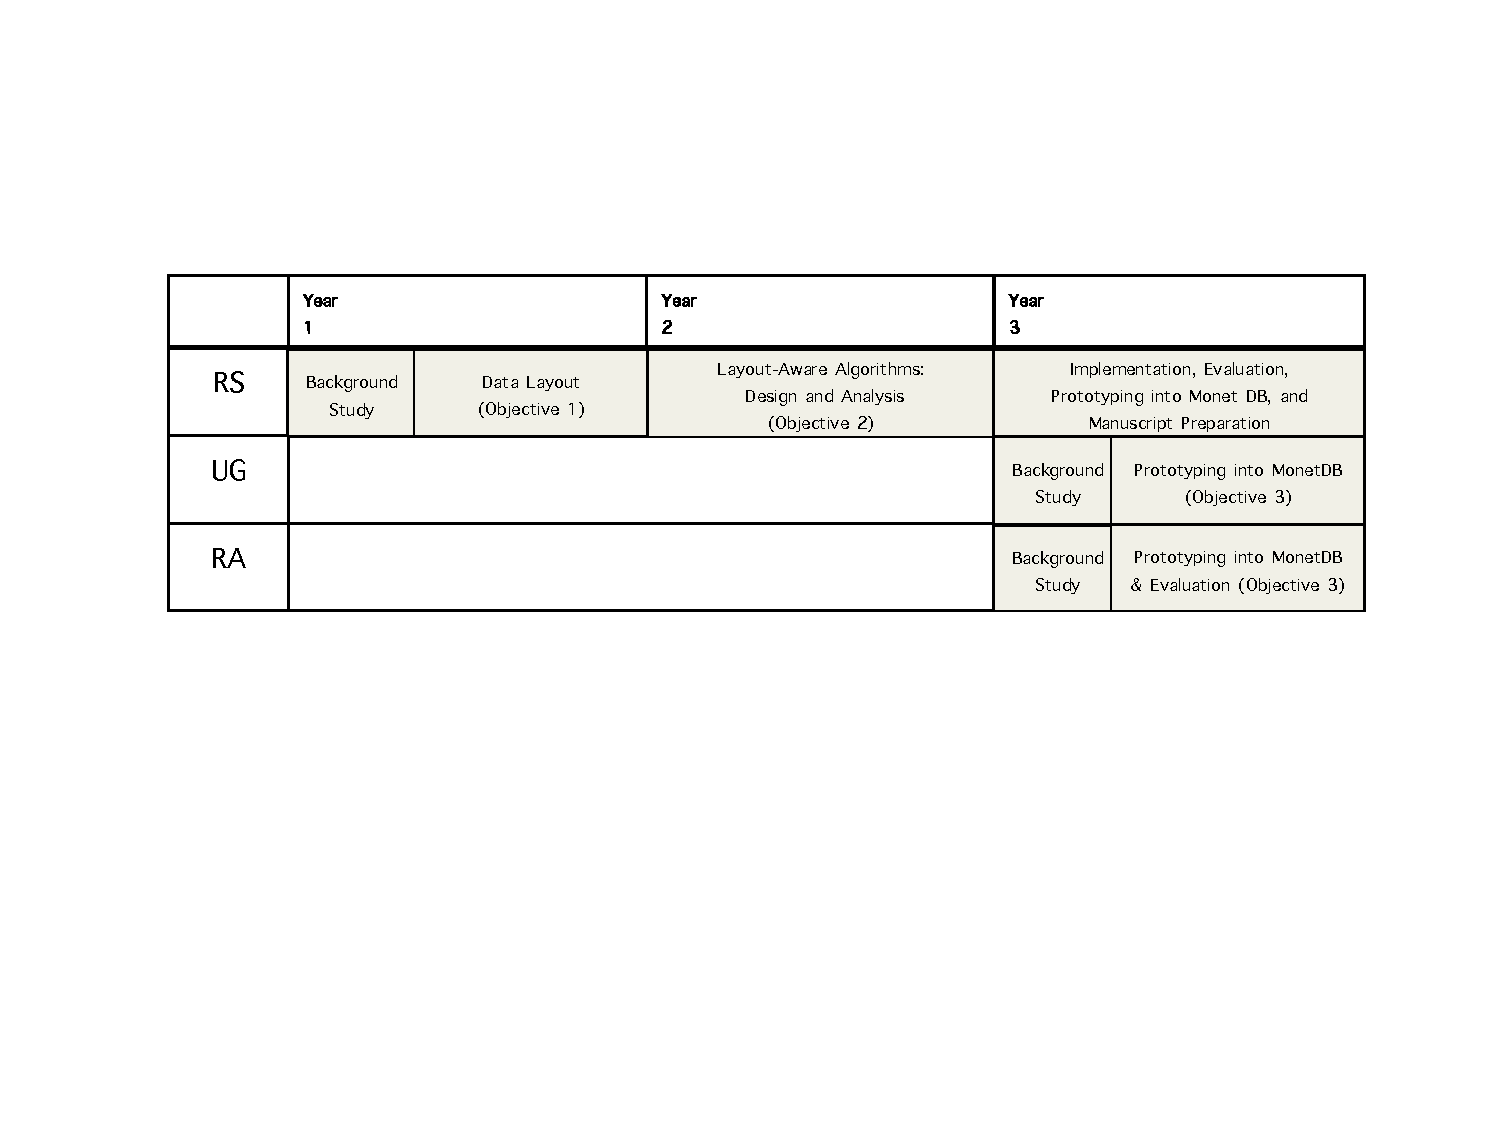
\includegraphics[width=15cm]{figs/GanttChart}
%\caption{Research Plan}
%\label{fig:plan}
%\vspace{-2ex}
%
%\end{figure}


\setlength{\bibsep}{0.0pt}

{%\footnotesize`
\small
% \bibliographystyle{abbrv}
%\bibliographystyle{abbrvnat}
%\bibliographystyle{plainnat}
\bibliographystyle{unsrtnat}
 \bibliography{0-BOLD-bibdoc,1-sparkpaper}
}

%%---------------------%%
\end{document}
%%---------------------%%
